\section{Resultados Experimentais}

\subsection{Etapa I: Validação da Odometria RK2}
% TODO: Analisar os resultados da Tabela~\ref{tab:etapa1_odometria}, Figura~\ref{fig:etapa1_trajetorias} e Figura~\ref{fig:etapa1_erros} para as 3 trajetorias (reta, arco circular e percurso composto em "S").

\begin{table}[htbp]
\centering
\caption{Métricas de erro da odometria RK2 em relação ao \textnormal{\textit{ground truth}} na Etapa I.}
\label{tab:etapa1_odometria}
\setlength{\tabcolsep}{3.5pt}
\resizebox{\columnwidth}{!}{%
\begin{tabular}{lccccc}
\toprule
\textbf{Trajetória} & \textbf{Comp. (m)} & \textbf{$\text{RMSE}_p$ (m)} & \textbf{$e_p(t_f)$ (m)} & \textbf{$\text{RMSE}_\theta$ ($^\circ$)} & \textbf{$e_\theta(t_f)$ ($^\circ$)} \\
\midrule
Linha Reta (5 m)        & 4,99 & 0,0039 & 0,0061 & 0,05 & 0,04 \\
Arco Circular ($R_c=1$ m) & 6,26 & 0,0042 & 0,0055 & 0,23 & 0,31 \\
Percurso Composto (``S'') & 4,99 & 0,0036 & 0,0039 & 0,17 & 0,04 \\
\bottomrule
\end{tabular}%
}
\end{table}


\begin{figure*}[t]
\centering
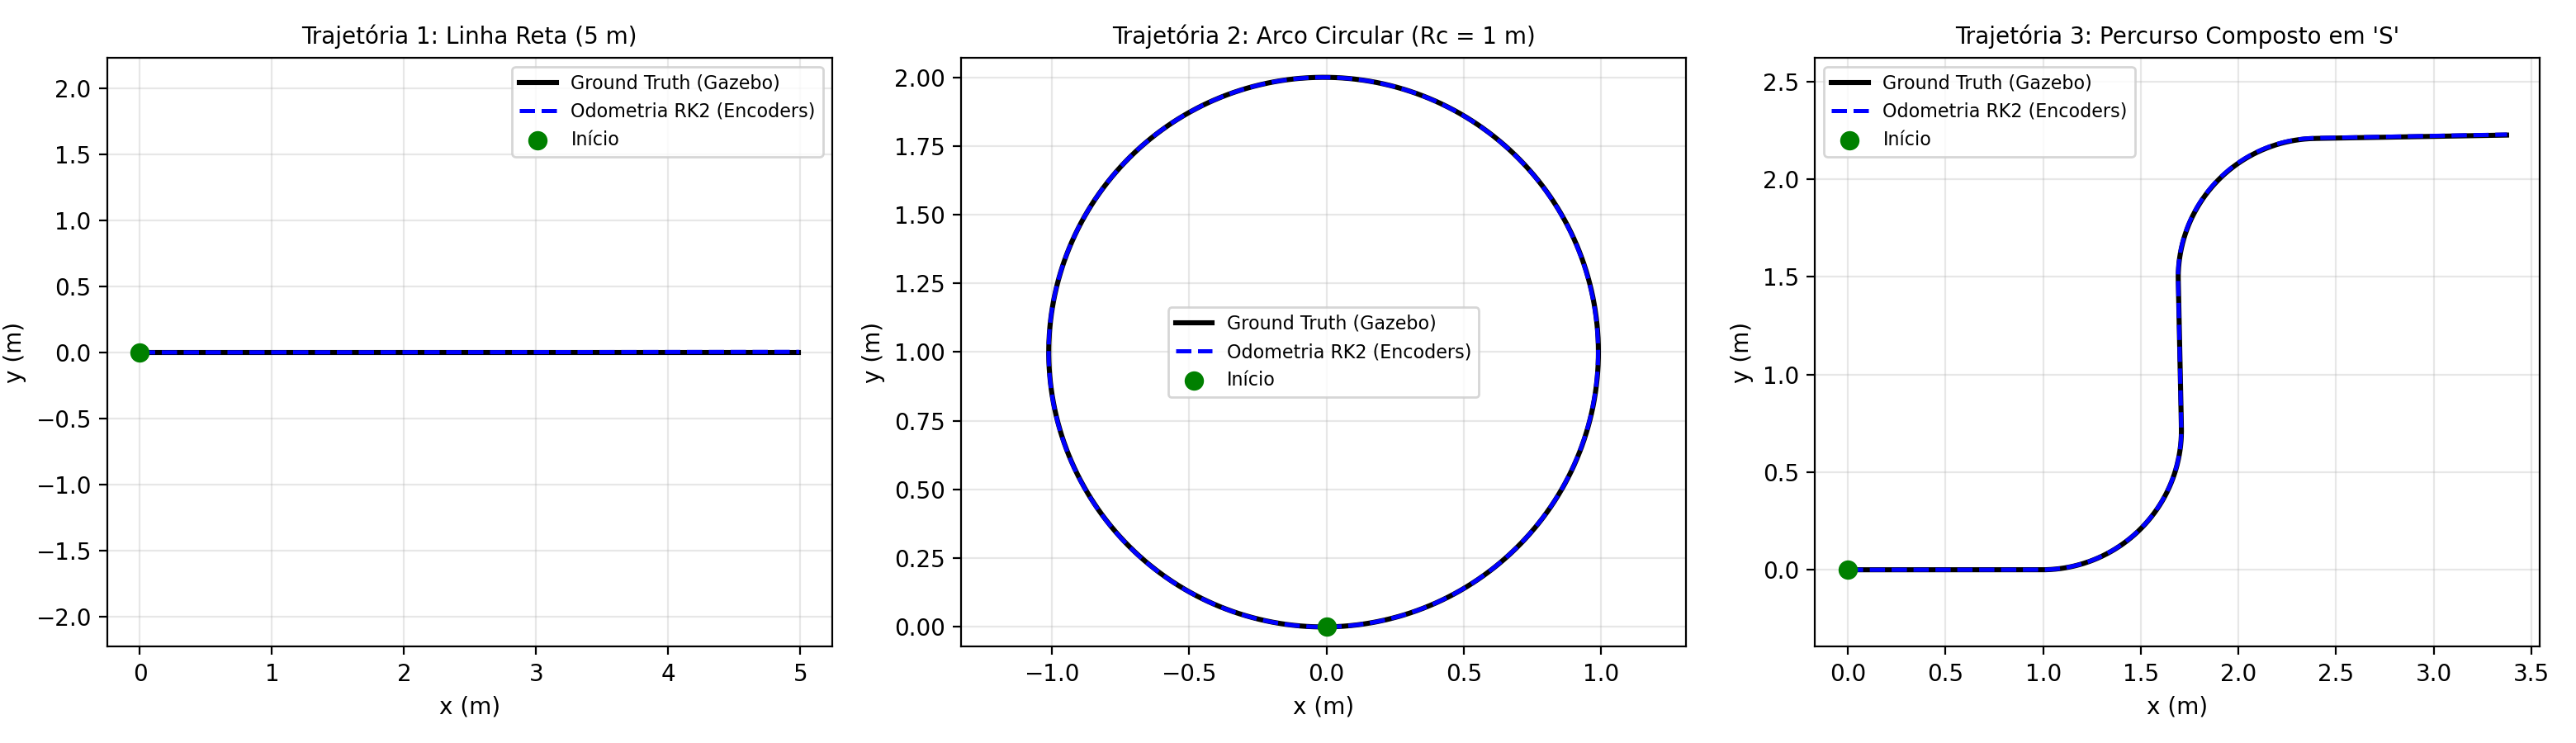
\includegraphics[width=\textwidth]{fig1_etapa1_trajetorias.png}
\caption{Comparação entre as trajetórias estimadas pela odometria RK2 e o \textit{ground truth} do simulador na Etapa~I.}
\label{fig:etapa1_trajetorias}
\end{figure*}

\begin{figure*}[t]
\centering
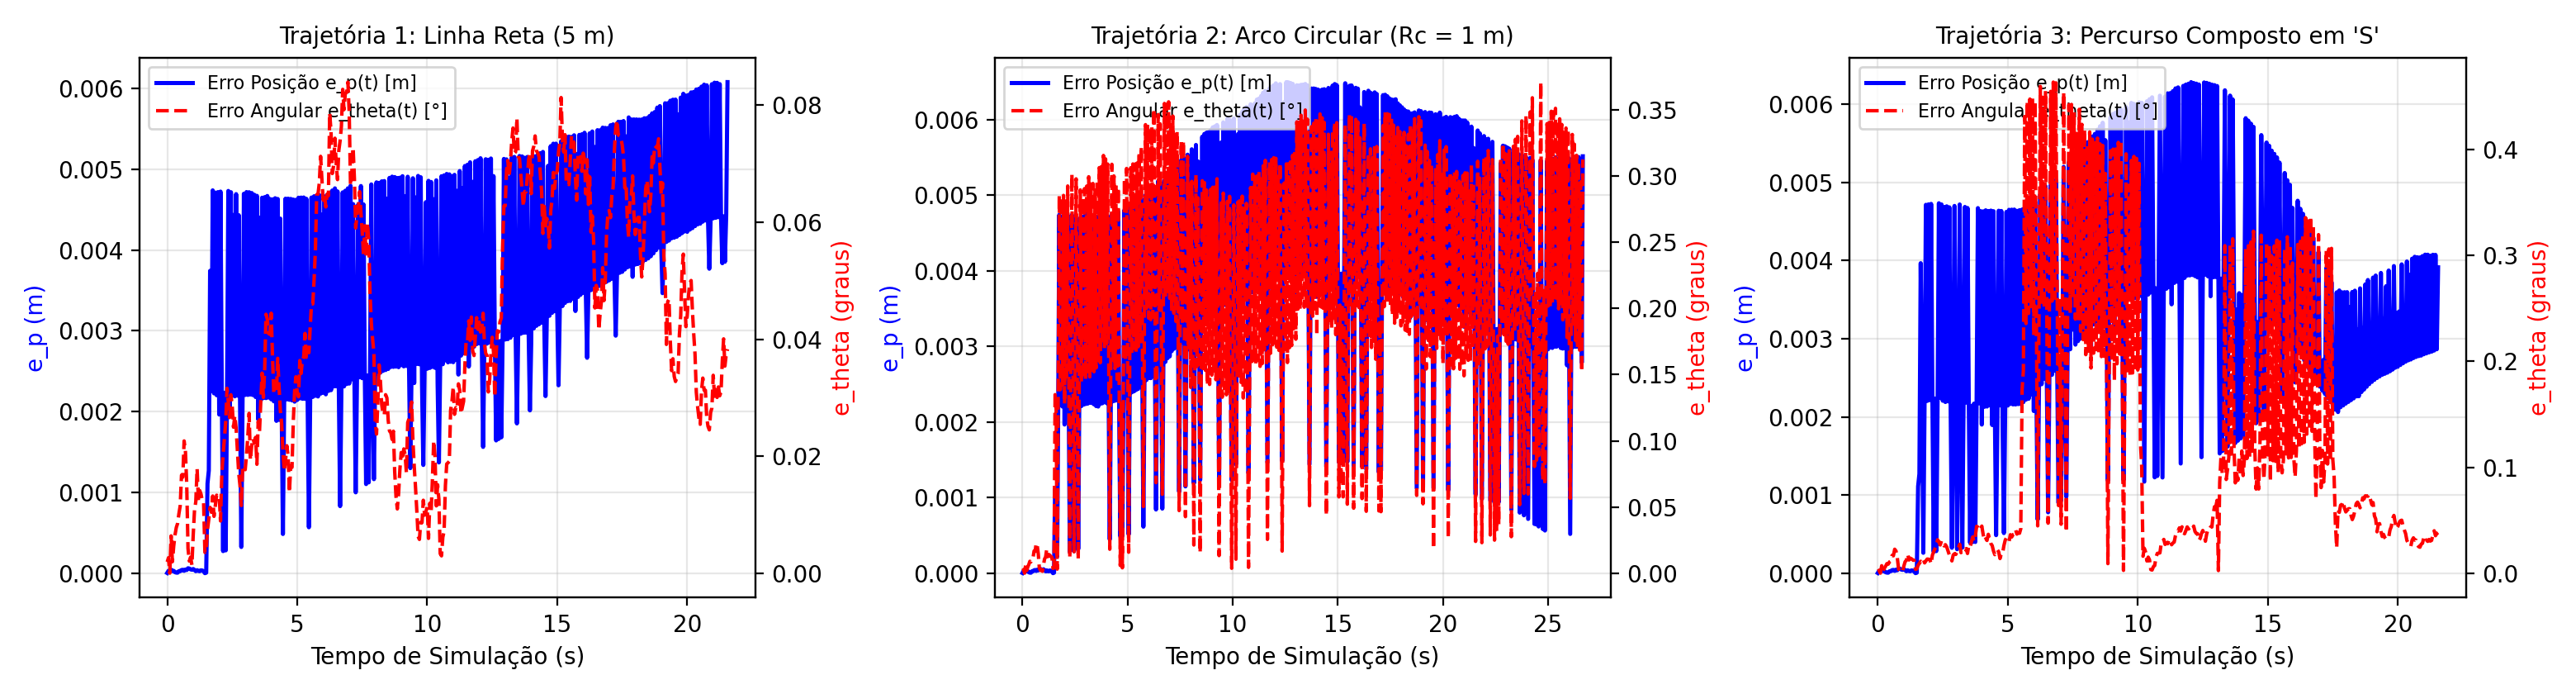
\includegraphics[width=\textwidth]{fig2_etapa1_erros.png}
\caption{Evolução temporal dos erros de posição $e_p(t)$ e orientação $e_\theta(t)$ na Etapa~I.}
\label{fig:etapa1_erros}
\end{figure*}

\subsection{Etapa II: Comparação APF vs. Bug2 nos Cenários A, B e GNRON}
% TODO: Analisar a Tabela~\ref{tab:comparacao_p6} e a Figura~\ref{fig:etapa2_cenarios} (N = 5 sementes, media +/- desvio padrao) destacando o comportamento de cada metodo nos Cenarios A, B e GNRON.

\begin{table*}[t]
\centering
\caption{Comparação quantitativa entre APF e Bug2 nos cenários experimentais ($N = 5$ execuções, sementes 42--46, média $\pm$ desvio padrão).}
\label{tab:comparacao_p6}
\setlength{\tabcolsep}{4pt}
\resizebox{\textwidth}{!}{%
\begin{tabular}{llcccccccc}
\toprule
\textbf{Cenário} & \textbf{Método} & \textbf{Sucesso (\%)} & \textbf{Colisões} & \textbf{$L_{\text{traj}}$ (m)} & \textbf{$T_{\text{tot}}$ (s)} & \textbf{$d_{\min}$ (m)} & \textbf{Bloqueios (\%)} & \textbf{$e_p(t_f)$ (m)} & \textbf{$d_{\text{meta}}$ (m)} \\
\midrule
Cenário A (Esparsos) & APF & 100\% & 0 & $10{,}01 \pm 0{,}00$ & $33{,}4 \pm 0{,}1$ & $0{,}28 \pm 0{,}00$ & 0\% & $0{,}0060 \pm 0{,}0027$ & $0{,}20 \pm 0{,}01$ \\
Cenário A (Esparsos) & Bug2 & 100\% & 0 & $9{,}68 \pm 0{,}02$ & $37{,}2 \pm 0{,}2$ & $0{,}36 \pm 0{,}00$ & 0\% & $0{,}0098 \pm 0{,}0033$ & $0{,}20 \pm 0{,}01$ \\
\midrule
Cenário B (Armadilha ``U'') & APF & 0\% & 0 & $3{,}05 \pm 0{,}00$ & $13{,}2 \pm 0{,}0$ & $0{,}47 \pm 0{,}00$ & 100\% & $0{,}0005 \pm 0{,}0006$ & $3{,}14 \pm 0{,}00$ \\
Cenário B (Armadilha ``U'') & Bug2 & 100\% & 0 & $12{,}25 \pm 0{,}02$ & $45{,}9 \pm 0{,}1$ & $0{,}38 \pm 0{,}00$ & 0\% & $0{,}0096 \pm 0{,}0022$ & $0{,}20 \pm 0{,}01$ \\
\midrule
Cenário GNRON & APF & 0\% & 0 & $5{,}65 \pm 0{,}00$ & $22{,}6 \pm 0{,}0$ & $0{,}80 \pm 0{,}00$ & 100\% & $0{,}0018 \pm 0{,}0012$ & $0{,}35 \pm 0{,}00$ \\
Cenário GNRON & Bug2 & 100\% & 0 & $5{,}81 \pm 0{,}00$ & $17{,}2 \pm 0{,}0$ & $0{,}66 \pm 0{,}00$ & 0\% & $0{,}0039 \pm 0{,}0007$ & $0{,}19 \pm 0{,}00$ \\
\bottomrule
\end{tabular}%
}
\end{table*}


\begin{figure*}[t]
\centering
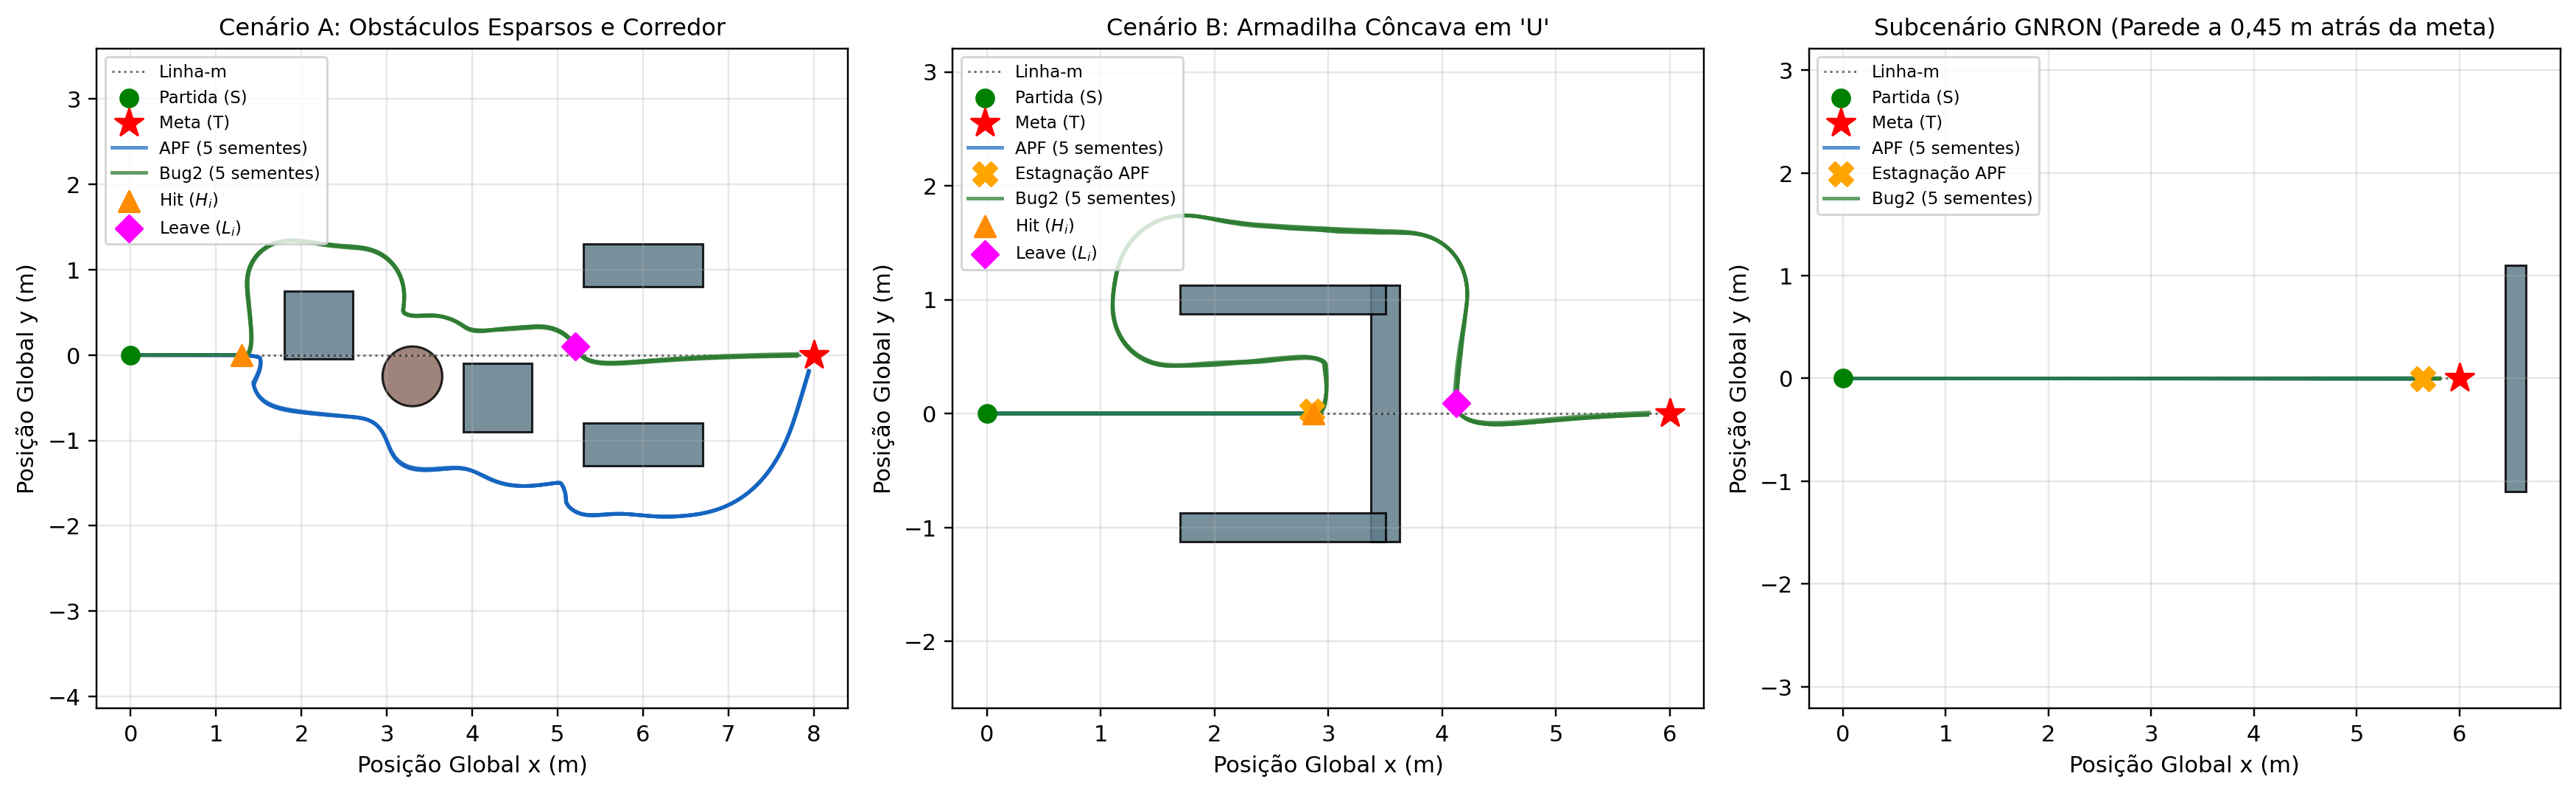
\includegraphics[width=\textwidth]{fig3_etapa2_comparacao_cenarios.png}
\caption{Trajetórias executadas (5 sementes) pelos métodos APF e Bug2 nos Cenários~A, B e no Subcenário GNRON.}
\label{fig:etapa2_cenarios}
\end{figure*}

\subsection{Estudo Paramétrico do APF e Limiar GNRON}
% TODO: Analisar a Figura~\ref{fig:etapa2_parametrico}:
% - Sensibilidade a (rho_0, k_rep) no Cenario A (colisoes na configuracao Fraco com d_min = 0,20 m vs. convergencia sem colisoes nas demais).
% - Efeito de rho_0 sobre o fenomeno GNRON (convergencia com rho_0 = 0,35 m < 0,45 m e estagnacao para rho_0 >= 0,80 m).

\begin{figure*}[t]
\centering
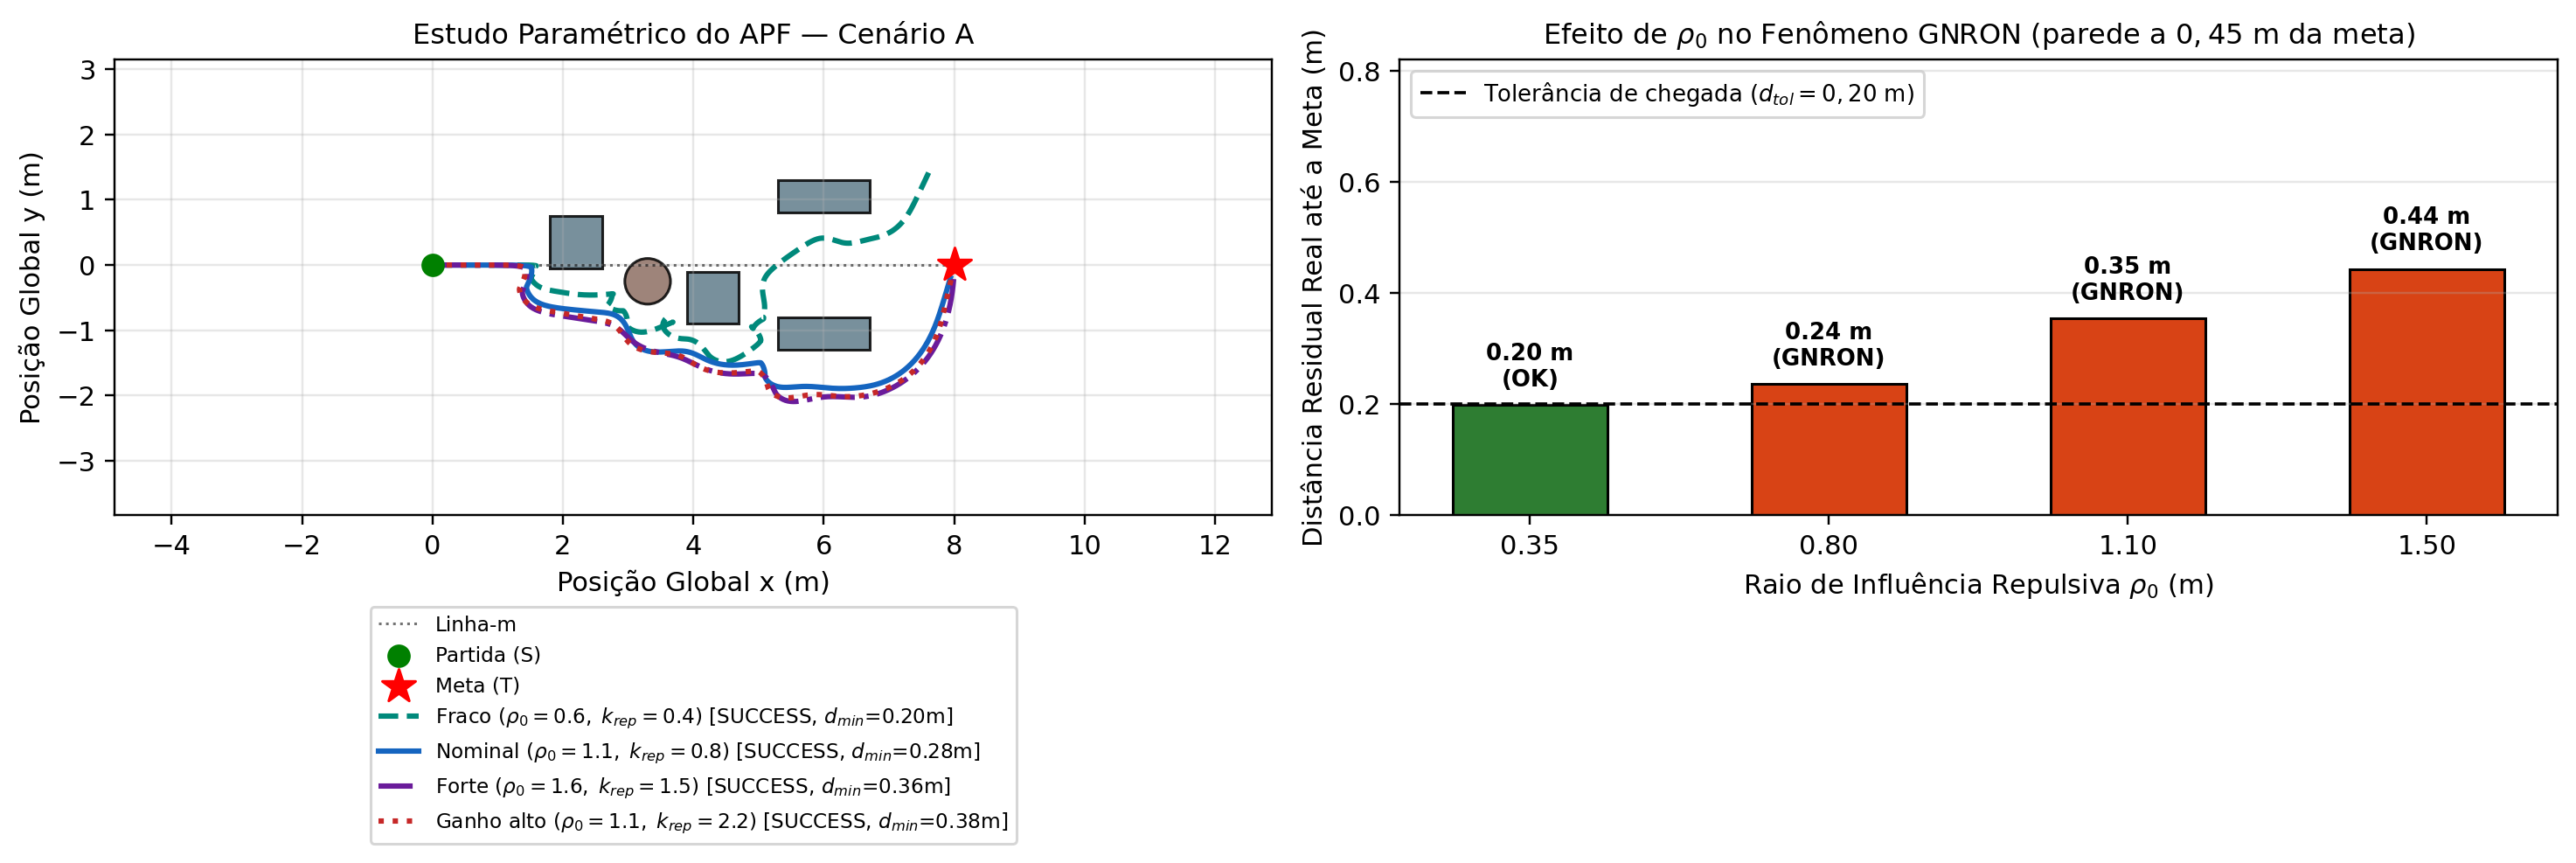
\includegraphics[width=\textwidth]{fig4_etapa2_estudo_parametrico.png}
\caption{Estudo paramétrico do APF no Cenário~A (esquerda) e efeito do raio de influência repulsiva $\rho_0$ no fenômeno GNRON (direita).}
\label{fig:etapa2_parametrico}
\end{figure*}
